%!TEX root = ../template.tex
%%%%%%%%%%%%%%%%%%%%%%%%%%%%%%%%%%%%%%%%%%%%%%%%%%%%%%%%%%%%%%%%%%%%
%% chapter3.tex
%% NOVA thesis document file
%%
%% Chapter with a short latex tutorial and examples
%%%%%%%%%%%%%%%%%%%%%%%%%%%%%%%%%%%%%%%%%%%%%%%%%%%%%%%%%%%%%%%%%%%%

\typeout{NT FILE chapter3.tex}%

\chapter{Related Work}
\label{cha:related-work}

In this chapter we will discuss relevant references more closely related to the objectives and contributions specifically expected for our planned dissertation. These topics are organized in the following way: section \ref{sec:rel_work_dl_scale_consensus} presents an analysis of the consensus plane and scalability approaches on permissionless blockchains; section \ref{sec:rel_work:dl_ds} discusses chained structures, the DAG model and other techniques to increase performance; section \ref{sec:rel_work:adversary_model-consensus-consistency} presents the adversary model for permissionless \gls{DL}s with an analysis of different consensus types and consistency guarantees; section \ref{sec:rel_work:sybil_committees} relates to multiple element committees and how to perform a sybil resistant election; section \ref{sec:rel_work:cup} introduces the \gls{CUP} model as a way to apply classical consensus mechanisms to permissionless systems with unknown participants; and in section \ref{sec:rel_work:critical_analysis} we perform a critical analysis of all the enumerated topics of this chapter.

\section{Decentralized Ledgers, Scale and Consensus Planes}
\label{sec:rel_work_dl_scale_consensus}

\subsection{Consensus Planes in Permissionless Blockchains}


As introduced before, permissioned blockchains are unsuitable for permissionless operation. First of all, they become less efficient when the number of nodes increase significantly, which corresponds to large-scale settings for cryptocurrency ecosystems, such as Bitcoin \cite{bitcoin} or Ethereum \cite{ethereum}. In another relevant perspective, they reach consensus based on a voting approach, that requires to control and possibly authenticate in order to resist sybil attacks \cite{sybil_attack}, namely collusion of faulty nodes. 

Some recent proposals of permissionless blockchains leverage the benefits of \gls{BFT} algorithms while also using \gls{PoW} to allow any node to be part of the system. This type of blockchains are based on hybrid consensus approaches. The main idea is that they can mix the two types of algorithms.
% 
% Bitcoin-NG [], for example, aims to provide a more scalable version of Bitcoin. The idea is to use a leader-based Byzantine consensus algorithm to order blocks of transactions. But to deal with the fact that any node can be part of the blockchain, Bitcoin-NG uses PoW to elect the leader. This use of PoW allows the existence of temporary forks, as happens in Bitcoin’s blockchain.
% 
% 
% PeerCensus [X69] (used to support a cryptocurrency called Discoin) and Hybrid-Chain  [X132] are based on a similar idea as above. They both use PoW to limit the rate at which nodes can join the blockchain, and run a Byzantine consensus algorithm among the blockchain nodes to order blocks. Again, the possibility of temporary forks remains. The Hybrid Consensus experimental resulsts show conditions in which a permissionless consensus can satisfy the property of responsiveness, Ths notion is interesting and related to latency conditions for a transaction to be confirmed as a function of the network delay. The authors prove that permissionless consensus is impossible in partially synchronous models, and that the proposed hybrid consensus is responsive (by leveraging a PoW base consensus layer).
% 
% Byzcoin [ ] is also based in a variation of Byzantine consensus for ordering and PoW for defining the committee of nodes that run the consensus [X100]. The authors introduce two interesting ideas to address performance. First, they substitute PBFT’s vectors of MACs by signatures, using a collective signing protocol (where nodes jointly cooperate to produce signatures), to avoid the leader to check O(n) signatures during consensus processing. They also use the notion of communication trees from multicast protocols, with the goal of reduction the number of sent messages.
% 
% Algorand is also designed as a cryptocurrency ecosystem, introducing new mechanisms, not based on PoW [X87]. The design model considers weighted users, i.e., where the voting power of each node depends on the amount of money it holds in the chain, with similarities with a PoS consensus model. At the same time it implements consensus by committee, where only a subset of the nodes (committee) run the Byzantine consensus algorithm, with a consequent reduction of the number of messages exchanged. An interesting idea here is that the committee members are chosen randomly, but the probability of a node being chosen is not constant and depends on its weight. Algorand also uses a cryptographic sortition scheme for committee members to be chosen in a private and non-interactive way (i.e., without communication). The goal is to make it harder for adversaries to do denial of service attacks against these nodes. Finally, the system uses participant replacement again to mitigate denial of service attacks. The idea is that once a committee member sends a message, it stops being a member, so it is no longer useful to do denial of service against it.
% 
% Solida [ ] was inspired by Byzcoin and Hybrid consensus [X6]. In this case transactions are ordered by a committee using a variant of the PBFT algorithm with a committee-model and leader-based consensus. The number of members of the committee is fixed. When a new member joins, the oldest leaves. To join to the committee a node must present a PoW and, when it does so, then it becomes the leader. If two nodes obtain a PoW concurrently, a leader election protocol must be executed to select which one becomes the leader. With this approach, it is avoided the creation of temporary forks.
% 
% Omniledger [ ] was designed, in some sense, to use a combination of mechanisms inspired above in the Byzcoin, but using a sharding model for better address scale conditions. More recent solutions that want to improve scalability and performance are also relevant. 










\begin{table}[ht]
\tiny
\centering
\begin{tabular}{|>{\centering\arraybackslash}m{2cm}|>{\centering\arraybackslash}m{1.3cm}|>{\centering\arraybackslash}m{1.2cm}|>{\centering\arraybackslash}m{1.1cm}|>{\centering\arraybackslash}m{1.1cm}|>{\centering\arraybackslash}m{1.1cm}|>{\centering\arraybackslash}m{1.1cm}|} 
\cline{2-6}
\multicolumn{1}{l|}{} & \multicolumn{5}{c|}{\textbf{\textbf{Consensus Plane}}} & \multicolumn{1}{l}{} \\ 
\cline{2-7}
\multicolumn{1}{c|}{} & \textbf{Mechanism}       & \textbf{Participants} & \textbf{Resiliency} & \textbf{Committee Type} & \textbf{Committee Sybil-Resistant} & \textbf{Smart Contracts} \\ 
\hline
\textbf{Bitcoin} \cite{bitcoin} & PoW & All & 51\% & - & - & \cmark \\
\textbf{Ethereum} \cite{ethereum} & PoS & All & 51\% & - & - & \cmark \\
\textbf{Bitcoin NG} \cite{bitcoin-ng} & PoW & All & 51\% & - & - & \cmark \\
\textbf{PeerCensus} \cite{peercensus} & PoW, PBFT & Committee & $3f + 1$ & Elected & \xmark & \xmark \\
\textbf{ByzCoin} \cite{byzcoin} & PoW, PBFT & Committee & $3f + 1$ & Elected & \xmark & \xmark \\
\textbf{OmniLedger} \cite{omniledger} & PoW, PBFT & Committee & $3f + 1$ & Elected & \cmark & \xmark \\
\textbf{Algorand} \cite{algorand, algorand_white_paper} & PPoS & Committee & 51\% & Elected & \cmark & \cmark \\
\textbf{Solida} \cite{solida} & PoW, PBFT & Committee & $3f + 1$ & Elected & \cmark & \xmark \\
\textbf{Hybrid Consensus} \cite{hybrid_consensus} & PoW, PBFT & Committee & $3f + 1$ & Elected & \cmark & \xmark \\
\textbf{RapidChain} \cite{rapid_chain} & PoW & All & 51\% & - & - & \xmark \\
\textbf{Elastico} \cite{elastico} & PoW & All & 51\% & - & - & \xmark \\
\textbf{OHIE} \cite{ohie} & PoW & All & 51\% & - & - & \xmark \\
\textbf{Prism} \cite{prism} & PoW & All & 51\% & - & - & \xmark \\
\textbf{Blockmess} \cite{blockmess} & PoW & All & 51\% & - & - & \xmark \\
\textbf{Hashgraph} \cite{hashgraph} & PoW & All & 51\% & - & - & \xmark \\
\textbf{Blockmania} \cite{blockmania} & PoW & All & 51\% & - & - & \xmark \\
\textbf{SPECTRE} \cite{spectre_dag} & PoW & All & 51\% & - & - & \xmark \\
\textbf{IOTA} \cite{tangle_iota_dag} & PoW & All & 51\% & - & - & \xmark \\
\textbf{PHANTOM} \cite{phantom_dag} & PoW & All & 51\% & - & - & \xmark \\
\textbf{Meshcash} \cite{meshcash} & PoW & All & 51\% & - & - & \xmark \\
\textbf{GHOST} \cite{ghost} & PoW & All & 51\% & - & - & \xmark \\
\textbf{Conflux} \cite{conflux_dag} & PoW & All & 51\% & - & - & \xmark \\

\hline
\end{tabular}
\caption{Comparison of different consensus mechanisms in blockchain Platforms}
\label{tab:compare_blockchains}
\end{table}



% \begin{table}[ht]
% \tiny
% \centering
% \begin{tabular}{|>{\centering\arraybackslash}m{1.3cm}|>{\centering\arraybackslash}m{1.5cm}|>{\centering\arraybackslash}m{1.3cm}|>{\centering\arraybackslash}m{1.2cm}|>{\centering\arraybackslash}m{1.1cm}|>{\centering\arraybackslash}m{1.1cm}|>{\centering\arraybackslash}m{1.1cm}|>{\centering\arraybackslash}m{1.1cm}|>{\centering\arraybackslash}m{1.4cm}|>{\centering\arraybackslash}m{0.8cm}|} 
% \cline{3-7}
% \multicolumn{1}{l}{}          & \multicolumn{1}{l|}{} & \multicolumn{5}{c|}{\textbf{\textbf{Consensus Plane}}}                                                                                & \multicolumn{1}{l}{}     & \multicolumn{1}{l}{}        & \multicolumn{1}{l}{}   \\ 
% \cline{2-10}
% \multicolumn{1}{c|}{}         & \textbf{Model}        & \textbf{Mechanism}       & \textbf{Participants} & \textbf{Resiliency} & \textbf{Committee Type} & \textbf{Committee Sybil-Resistant} & \textbf{Smart Contracts} & \textbf{Membership control} & \textbf{Peer anonym.}  \\ 
% \hline
% \textbf{Bitcoin} \cite{bitcoin}              & Permissionless        & PoW                &       All                &         51\%            &        -                 &          -    &      \cmark       & Open model                  &           \cmark             \\
% \textbf{Bitcoin NG} \cite{bitcoin-ng}           & Permissionless        & PoW                &        All               &         51\%            &        -                 &          -      &     \cmark      & Open model                  &           \cmark             \\
% \textbf{Ethereum}  \cite{ethereum}           & Permissionless        & PoS                &      All                 &         51\%            &        -                 &          -     &     \cmark       & Open model                  &            \cmark            \\
% \textbf{ByzCoin}   \cite{byzcoin}           & Permissionless        & PBFT               &         Committee              &         $3f + 1$            &              Elected           &           \xmark       &    \xmark     & Open model                  &      \cmark          \\
% \textbf{OmniLedger}  \cite{omniledger}       & Permissionless        & PBFT               &         Committee              &         $3f + 1$            &              Elected           &           \cmark       &    \xmark     & Open model                  &            \cmark            \\
% \textbf{Algorand}  \cite{algorand, algorand_white_paper}           & Permissionless        & PPoS               &           Committee            &         51\%            &        Elected                 &          \cmark    &      \cmark       & Open model                  &           \cmark             \\
% \textbf{Blockmess}  \cite{blockmess}          & Permissionless        & PoW                &           All            &         51\%            &        -                 &          -    &      \xmark       & Open model                  &            \cmark            \\ 
% 
% % \textbf{Hyperledger Fabric} \cite{hyperleder_fabric}   & Permissioned          & Off-chain Services &         Committee              &        $3f + 1$             &               Deployed          &           \cmark      &     \cmark     & Private model               &         \xmark               \\
% % \textbf{Hyperledger Sawtooth} \cite{hyperledger_sawtooth, sawtooth_whitepaper} & Permissioned          & PBFT/PoET/ Others  &    All\tablefootnote{If using \gls{PoET}} / Committee\tablefootnote{If using \gls{PBFT}}             &       51\%$^1$/ $3f + 1^2$             & Deployed$^2$                     &           \cmark$^2$        &   \cmark     & Private model               &            \xmark            \\
% 
% % \textbf{Hyperledger Indy} \cite{hyperledger_indy}    & Permissioned          & RBFT               &            Committee           &          $3f + 1$           &               Deployed          &            \cmark     &    \xmark      & Private model               &           \xmark             \\
% % \textbf{Quorum}               & Permissioned          & Consortium         &         Committee              &          $3f + 1$           &                         &                &     \cmark      & Private model               &            \cmark            \\
% \hline
% \end{tabular}
% \caption{Comparison of different blockchain Platforms}
% \label{tab:compare_blockchains}
% \end{table}

% \todo{verificar se a tabel tem a coluna model, se é só para permissionless}

In table \ref{tab:compare_blockchains}, we present a comparative analysis between classical and research oriented permissionless blockchains focused on the consensus plane characteristics and support for smart contracts. The comparison is focused on different approaches for the consensus plane in which we explored the following characteristics: used consensus mechanism, the type of participation in the algorithm and the resiliency of the protocol.

As a result of this analysis it is possible to extract that classical permissionless blockchains tend to use a single hardcoded consensus mechanism, thus not dealing with the problem of using multiple consensus. With this approach, the performance of these systems is limited to the tradeoffs of the employed consensus mechanism which tends to be \gls{PoW} and \gls{PoS}. However, there are some solutions that try to mitigate these tradeoffs, Bitcoin-NG \cite{bitcoin-ng} is an example of a blockchain designed to scale and inspired in Bitcoin \cite{bitcoin} with the purpose of improving the scalability and throughput of this system which is only limited by the bandwidth of peers and propagation time of the network. Another approach consists of using a classical \gls{BFT} consensus mechanism like \gls{PBFT}, not so common in the permissionless model due to scalability issues but instead, applied to a committee of participants \cite{byzcoin, omniledger} known as a Hybrid Consensus. Following this approach, an election procedure of a committee is needed to be able to execute the consensus algorithm. Note that, this election should be periodically executed with security guarantees, namely a non-sybil election like the one performed by the Omniledger blockchain \cite{omniledger}. Additionally, we can also extract that systems that apply other scale-in or scale-out approaches tend to use \gls{PoW} as the consensus mechanism.
% On the other hand, permissioned blockchains imply access control and much reduced number on the participants. Therefore, blockchains of this type tend to offer the possibility of having multiple consensus (pluggable consensus) but they do not deal with the problem of scalability present on permissionless blockchains. Additionally, when using a classical \gls{BFT} consensus mechanism a committee is needed but in this case the problem of choosing a non-sybil committee is not applied due to the fact of it being determined and configured at deployment of the system.



% Tabela com permissionless e permissioned
% 
% Classical permissionless Bcs
% 
% Bcs | Model | Consensus Plane | Smart contract support | Membership control and participation | Peer Identification
% Bitcoin | permissionless | PoW using hash based mechanisms | support for scripts | open model | Anonymous
% Bitcoin NG
% Ethereum
% Bizzcoin
% ??Omniledger
% 
% cariz permissionless -> pow, pos
% cariz permissionned -> BFT or CFT
% 
% 
% ?? (Maybe) Recent research oriented bcs
% 
% permissioned -> implica access-control
% nenhuma bc permissionless lida com o problema de utilizar vários consensus

% tamanho letra - tabelas...: 30\%
% 
% coluna -> quem entra no consenso: all, committee (elected non-sybil or configured)
% -> resiliency -> 3f+1, 51\%
% -> committee organization - elected non-sybil ou configured/deployed
% 
% omniledger - non sybil committee

\subsection{Scalability Approaches in Permissionless Blockchains}

Together with the above solutions, the table \ref{tab:compare_scalability_blockchains} summarizes other approaches for permissionless blockcains in addressing scalability issues, together with relevant used mechanisms. % In these solutions we selected Parallel Chains (xcxvcxcvxvcxvcxvcx) [ ] [ ] [ ] …., DAG-based solutions using Blockless architectures [ ] [ ] [ ] [ ] or Block oriented proaches [ ] [ ] [ ] [ ].
In the next sections we will discuss more about these solutions, namely \gls{DAG} based blockchains, Sharding, Multichains and Parallel Chains.

\begin{table}[ht]
\tiny
\centering
\begin{tabular}{|>{\centering\arraybackslash}m{2.2cm}|>{\centering\arraybackslash}m{1.3cm}|>{\centering\arraybackslash}m{1cm}|>{\centering\arraybackslash}m{1.1cm}|>{\centering\arraybackslash}m{1.1cm}|>{\centering\arraybackslash}m{0.7cm}|>{\centering\arraybackslash}m{1.1cm}|>{\centering\arraybackslash}m{1cm}|>{\centering\arraybackslash}m{0.8cm}|>{\centering\arraybackslash}m{1cm}|} 
\cline{3-10}
\multicolumn{1}{l}{} & \multicolumn{1}{l|}{} & \multicolumn{1}{c|}{\textbf{\textbf{Scale-out}}} &
\multicolumn{7}{c|}{\textbf{\textbf{Scale-in}}} \\ 
\cline{2-10}
\multicolumn{1}{c|}{} & \textbf{Consensus} & \textbf{State-Sharding} & \textbf{Sharded Computations} & \textbf{Multiple Parallel Chaining} & \textbf{Blocks in main chain} & \textbf{DAG Blockless} & \textbf{DAG Block oriented} & \textbf{Hybrid Consensus} & \textbf{Flexible use of Consensus Plane} \\ 
\hline
\textbf{Bitcoin} \cite{bitcoin} & PoW & \xmark & \xmark & \xmark & \cmark & \xmark & \xmark & \xmark & \xmark \\
\textbf{Ethereum I} \cite{ethereum} & PoW & \xmark & \xmark & \xmark & \cmark & \xmark & \xmark & \xmark & \xmark \\
\textbf{Ethereum II} \cite{ethereum} & PoS & \xmark & \xmark & \xmark & \cmark & \xmark & \xmark & \xmark & \xmark \\
\textbf{Bitcoin NG} \cite{bitcoin-ng} & PoW & \xmark & \xmark & \xmark & \cmark & \xmark & \xmark & \cmark & \xmark \\
\textbf{PeerCensus} \cite{peercensus} & PoW, PBFT & \xmark & \xmark & \xmark & \cmark & \xmark & \xmark & \cmark & \xmark \\
\textbf{Hybrid Consensus} \cite{hybrid_consensus} & PoW, PBFT & \xmark & \xmark & \xmark & \cmark & \xmark & \xmark & \cmark & \xmark \\
\textbf{ByzCoin} \cite{byzcoin} & PoW, PBFT & \xmark & \xmark & \xmark & \cmark & \xmark & \xmark & \cmark & \xmark \\
\textbf{Solida} \cite{solida} & PoW, PBFT & \xmark & \xmark & \xmark & \cmark & \xmark & \xmark & \cmark & \xmark \\
\textbf{Algorand} \cite{algorand, algorand_white_paper} & PPoS & \xmark & \xmark & \xmark & \cmark & \xmark & \xmark & \xmark & \xmark \\
\textbf{OmniLedger} \cite{omniledger} & PoW, PBFT & \cmark & \cmark & \xmark & \cmark & \xmark & \xmark & \xmark & \xmark \\
\textbf{RapidChain} \cite{rapid_chain} & PoW & \cmark & \cmark & \xmark & \cmark & \xmark & \xmark & \xmark & \xmark \\
\textbf{Elastico} \cite{elastico} & PoW & \xmark & \cmark & \xmark & \cmark & \xmark & \xmark & \xmark & \xmark \\
\textbf{OHIE} \cite{ohie} & PoW & \xmark & \xmark & \cmark & \xmark & \xmark & \xmark & \xmark & \xmark \\
\textbf{Prism} \cite{prism} & PoW & \xmark & \xmark & \cmark & \xmark & \xmark & \xmark & \xmark & \xmark \\
\textbf{Blockmess} \cite{blockmess} & PoW & \xmark & \xmark & \cmark & \xmark & \xmark & \xmark & \xmark & \xmark \\
\textbf{Hashgraph} \cite{hashgraph} & PoW & \xmark & \xmark & \cmark & \xmark & \cmark & \xmark & \xmark & \xmark \\
\textbf{Blockmania} \cite{blockmania} & PoW & \xmark & \xmark & \cmark & \cmark & \xmark & \xmark & \xmark & \xmark \\
\textbf{SPECTRE} \cite{spectre_dag} & PoW & \xmark & \xmark & \xmark & \cmark & \xmark & \cmark & \xmark & \xmark \\
\textbf{IOTA} \cite{tangle_iota_dag} & PoW & \xmark & \xmark & \xmark & \cmark & \cmark & \xmark & \xmark & \xmark \\
\textbf{PHANTOM} \cite{phantom_dag} & PoW & \xmark & \xmark & \xmark & \cmark & \xmark & \cmark & \xmark & \xmark \\
\textbf{Meshcash} \cite{meshcash} & PoW & \xmark & \xmark & \xmark & \cmark & \xmark & \cmark & \xmark & \xmark \\
\textbf{GHOST} \cite{ghost} & PoW & \xmark & \xmark & \xmark & \cmark & \xmark & \cmark & \xmark & \xmark \\
\textbf{Conflux} \cite{conflux_dag} & PoW & \xmark & \xmark & \xmark & \cmark & \xmark & \cmark & \xmark & \xmark \\
\hline
\end{tabular}
\caption{Scalability approaches for different permissionless blockchains}
\label{tab:compare_scalability_blockchains}
\end{table}

% \todo{dags e parallel tem em vista otimizar o througput spearando o consenso da disseminação na rede. no caso das dags a ideia é fazer com que o consenso seja executado sem rondas de communication. no caso de paralelas nem sempre é endereaç~do com expceção.}

As a result of this analysis, we can extract that \gls{DL}s that use approaches like \gls{DAG}s or parallel chains have the objective to optimize throughput by separating consensus from network dissemination. In the case of \gls{DAG}s, the idea is for the consensus to be executed without any external communication between nodes. However, in the case of parallel chains this approach is not always addressed, with Prism \cite{prism} being an exception.

Additionally, as presented on the table, solutions employing a Hybrid Consensus restrict the use of the supported consensus mechanisms in the sense that one of them is used for committee election and the other one is for executing the consensus of blocks. This is captured by the table in the sense that there are no solutions that employ a Hybrid and Flexible use of the consensus plane, which we will address in our approach.



\section{Decentralized Ledgers and Data Structures}
\label{sec:rel_work:dl_ds}

% In this section we will discuss Decentralized Ledgers focusing in the weight use applied in chained structures. % and also how the \gls{DAG} model can be used to

% A Decentralized Ledger corresponds to a system in which data is replicated and accessible across many nodes. As mentioned in section \ref{sec:background:decentralized_ledgers}, a \gls{DL} solves the consensus problem under the \gls{BFT} model in the permissionless setting. As a result, a \gls{DL} can be represented by three components: a Sybil Resistant Committee, an Intermidi

% (Pedro)

\subsection{Chained Structures}
\label{subsec:dl_ds:weight_chained_struct}

Chained structures or blockchain is the simplest and most popular implementation of a \gls{DL}. In this kind of structures, a \gls{DL} is modeled as a set of blocks in which a block contains 2 main fields: \textbf{\textit{prev}} - a reference to the previous block in the chain, generally a hash of the block; and \textbf{\textit{data}} - represents the data stored in the block which in most blockchains, the data are transactions. In figure \ref{fig:blockchain-block-struct} is presented the structure of a block.

\begin{figure}[h]
    \centering
    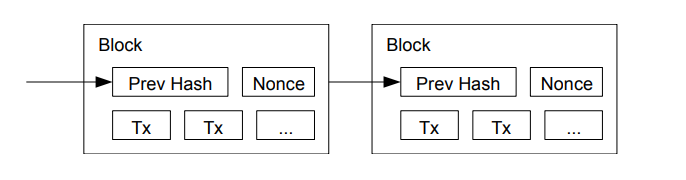
\includegraphics[scale=0.5]{Chapters/Figures/block-struct.png}
    \caption{Bitcoin \cite{bitcoin} Block structure}
    \label{fig:blockchain-block-struct}
\end{figure}

As mentioned in the last chapter in section \ref{sec:background:decentralized_ledgers}, a \gls{DL} needs to solve the consensus problem in order to be able to add new information to the ledger which in this case corresponds to adding a new block to the chain. However, in this kind of systems, some participants may have a different view of the system state or malicious intents which could lead to inconsistencies on the ledger, namely \textbf{forks}.
As a result, this structure forms a tree in which the root corresponds to the \textit{genesis} block, i.e. the first block on the chain and each chain (an ordered set of blocks with the first block being the \textit{genesis} one) is assigned a \textbf{weight}. Since only one chain can contain blocks that can be finalized, the weight is used to determine the chain which has the biggest weight - \textbf{heaviest chain}. In fact, the chain weight can be measured in different ways, but the most common is called the \textbf{longest chain} rule, applied in Bitcoin \cite{bitcoin} and consists of finding the chain that has the greater sum of weights of all the blocks that are contained in it.

In Bitcoin \cite{bitcoin}, a fork is created when two nodes accept a block and broadcast it for the same position in the ledger. In fact, the probability of a fork is proportional to the rate of proposed blocks and inversely proportional to the time required to disseminate a block \cite{bitcoin_info_network_propagation}. As a result, if there are multiple blocks being proposed compared with their propagation time, the probability of those blocks referencing the same previous block is much higher and performance suffers greatly. This means that for the system to maintain certain safety guarantees, it is needed to lower the block creation rate which increases the confirmation time of transactions and thus, reducing the throughput of the system.
% In Bitcoin \cite{bitcoin}, a fork is created when two nodes accept a block and broadcast it for the same position in the ledger, i.e. the two blocks have the same previous block. Technically, this inconsistency is related to the fact that two nodes have a different state of the ledger (ex. out-of-date) which influences the validation of a block and transactions. Additionally, as opposed to the correct behavior of nodes although with different states, there are cases when a fork is created due to malicious nodes that accept invalid transactions, exploiting the Double Spending problem, i.e. referencing input transactions that were already used. In fact, the probability of a fork is proportional to the rate of proposed blocks and inversely proportional to the time required to disseminate a block \cite{bitcoin_info_network_propagation}. As a result, if there are multiple blocks being proposed compared with their propagation time, the probability of those blocks referencing the same previous block is much higher and performance suffers greatly. This means that for the system to maintain certain safety guarantees, it is needed to lower the block creation rate which increases the confirmation time of transactions and thus reducing the throughput of the system. However, forks can still happen due to network partitions between nodes and so, the system must guarantee that it eventually gets to a common state that is consistency across all replicas even in the presence of forks, thus requiring to resolve forks.

% Eventually, during a fork, one of the chains will become longer than the others and the partitions of nodes that did not adopt that chain will switch to it. This is ensured because miners will only propose (mine) blocks that they believe to be correct, i.e. blocks that belong to the heaviest chain, thus enforcing the rule of the longest chain, otherwise the block could be discarded and all the work done will be useless. Also, a correct behaviour of nodes is a guarantee of the possibility to have revenue for mining. Therefore, the fork will be eventually considered to be resolved and all replicas are consistent up to the head of that chain. The blocks that belong to the discarded chains will be invalidated and are called as \textit{orphan blocks}. This leads us to the concept of finalization of blocks. A block is finalized when it belongs to a chain that has a weight grater than all others by a certain parameter, referred as \textbf{finalization depth}.

\begin{figure}[h]
    \centering
    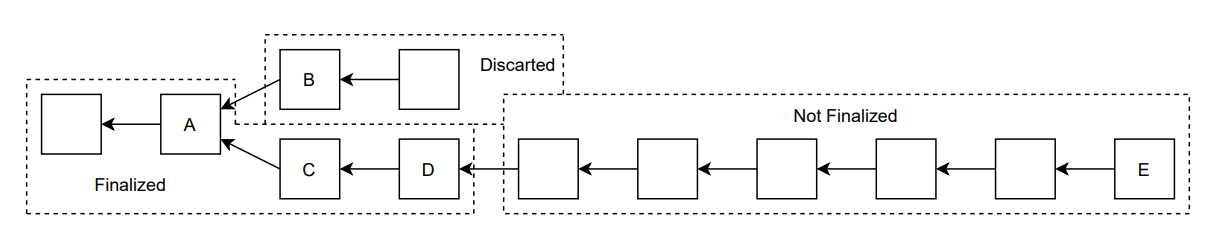
\includegraphics[scale=0.4]{Chapters/Figures/blockchain-fork.png}
    \caption{Blockchain fork (from \cite{blockmess})}
    \label{fig:blockchain-fork}
\end{figure}

In figure \ref{fig:blockchain-fork}, is presented a fork on the Bitcoin blockchain after block $A$ resulting in two chains initiated by blocks $B$ and $C$ which cannot be finalized. When block $E$ is appended, blocks $C$ and $D$ can be finalized because the fork initiated by $C$ is longer than the other one by 6 blocks which corresponds to the \textbf{finalization depth}. This ensures that the fork started by $B$ cannot become the longest chain because miners will only propose blocks that they believe to be correct, i.e. blocks that belong to the heaviest chain, thus enforcing the rule of the longest chain. Since a fork can occur after block $D$, any block that follows $D$ cannot be finalized because other chain could become the longest chain.

On the other hand, in Bitcoin-NG \cite{bitcoin-ng}, the operation of the blockchain is different from Bitcoin in the sense that are introduced two kinds of blocks:
\begin{itemize}
    \item \textbf{key blocks}: Blocks that are used to elect a leader which corresponds to the next proposer of the next batch of Micro-blocks. As in Bitcoin, these kind of blocks follow the same approach in the sense that they need to be mined in order to be appended to the chain.
    \item \textbf{Micro-blocks}: Blocks used to record and append transactions to the ledger by the current leader. This kind of blocks do not need to be mined as they are related to the current leader (the previous key block) in order to be valid.
\end{itemize}

Since micro-blocks do not need to be mined, the append rate of those blocks are much higher which increases the throughput of transactions. However, forks can still happen in this system and as in Bitcoin, nodes choose to mine on the chain with most work.

\begin{figure}[h]
    \centering
    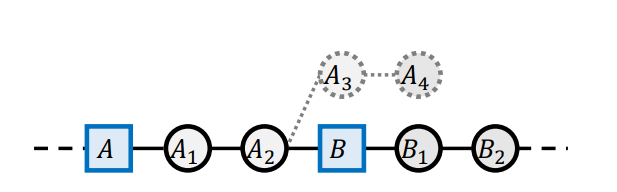
\includegraphics[scale=0.45]{Chapters/Figures/blockchain-fork-bitcoin-ng.png}
    \caption{Blockchain fork in Bitcoin-NG \cite{bitcoin-ng}}
    \label{fig:bitcoin-ng-fork}
\end{figure}

In figure \ref{fig:bitcoin-ng-fork}, is presented a fork in the Bitcoin-NG platform. In this example, node $A$ mined a key block and appended two micro-blocks, $A_1$ and $A_2$. Node $B$ mined a key block referencing $A_2$, thus creating a fork and enforcing a leader change. In this case, the chain initiated by a key-block from $B$ wins and the micro-blocks $A_3$ and $A_4$ are discarded thus, resolving the fork.



\subsection{DAG Models}
\label{subsec:dl_ds:dag}

Although the blockchain is the most popular implementation of a \gls{DL}, there are some limitations that other implementations try to overcome, namely the throughput and scalability of the system. Based on this, alternative implementations % \cite{block_dag, tangle_iota_dag, conflux_dag, spectre_dag, phantom_dag}
relax properties and constraints of blockchains when referring to the block structure. This type of solutions form a \gls{DAG} structure which can be of two types \cite{sok}: \gls{DAG} Block oriented chains \cite{spectre_dag, phantom_dag, meshcash, ghost, conflux_dag} and \gls{DAG}-Blockless structures \cite{hashgraph, tangle_iota_dag}.

\subsubsection{DAG with Block oriented chains}

The \gls{DAG} model with Block oriented chains corresponds to a type of block graph that allows a block to reference a set of predecessor blocks. The main advantage of this structure over a blockchain (that only references a single previous block) is the possibility to incorporate the contents of all off-chain blocks (blocks that do not belong to the heaviest chain) that do not conflict with each other. With this, it is possible for nodes to validate and accept non conflicting transactions from blocks in different chains produced by a fork. To this purpose, an Inclusive Protocol is used as a method to define the set of accepted transactions. Therefore, blocks do not need to be linked in a single chain in order to be finalized thus, the block proposal rate is much higher and the negative impacts of forks can be reduced, namely the wasted resources used in mining blocks that turn to be invalid.

However, some solutions like \cite{block_dag, phantom_dag} are vulnerable to liveness attacks. In these cases, they perform a topological sort of blocks in order to get a total order of blocks and if the block proposal rate is high they are vulnerable to such attacks. Others, like \cite{spectre_dag} provide a weaker form of consistency in the sense that the system obtains a non-transitive partial order for any pair of blocks in the \gls{DAG}. With this, systems that follow this approach are limited as it is very difficult to support smart contracts without having a total order. Despite the weaker consistency model supported by those systems, this model is strong enough to support cryptocurrencies where users can trade tokens while the system needs to verify and mitigate Double Spending attacks.

\subsubsection{DAG with Blockless Data Structures}

There are other proposes \cite{aleph, hashgraph} that try to decouple data dissemination from the consensus mechanism which allows to improve scalability conditions. This approach is based on efficient implementations of \gls{DAG}s which allows to build simpler and efficient consensus mechanisms. In this type of \gls{DAG} based blockless implementations, instead of grouping transactions into blocks, transactions are linked in a way that form a \gls{DAG} graph. Then, every node can have the same graph structure and the consensus logic does not need to incur in a communication overhead because each node will only process its local view of the graph computing a total order without sending any messages.



% \subsection{Decoupling consensus from network-data dissemination}
% \label{subsec:dl_ds:decoupling_consensus}

% (BLOG MALKI) - pedir artigo ao prof


% \subsection{Sharding}
\subsection{Sharding, Multichains and Parallel chains}

\paragraph{Sharding}

One of the most practical way of achieving horizontal scalability is by using a technique known as Sharding. Sharding is based on the idea of partitioning the state of the system into multiple parts, which avoids the duplication of resources by all participating nodes, such as: communication, data storage and computation. Unlike regular blockchains, in this type of solutions \cite{sharding_survey, towards_scaling_via_sharding, elastico, omniledger, rapid_chain}, a set of nodes is responsible for a single part (shard) of the system, thus benefiting from parallelism to achieve full performance improvements while preserving the necessary security and decentralization of the system.
However, there are some issues when implementing such systems \cite{sharding_survey}, such as: \textit{intra-consensus safety} and \textit{cross-shard-atomicity}. Since the system is divided into multiple shards with each one independent from each other, the adversary can perform a coordinate attack to a single shard instead of the entire network in which the probability of success is much higher. To mitigate this problem, the election of nodes to different shards must be a result of a randomized process with sybil resistant properties \cite{sybil_attack}. The latter problem is encountered when processing cross-shard transactions in which the state from multiple shards needs to be merged. This point of convergence is extremely important and must be secured in order to guarantee the atomicity of these transactions. % Therefore, solutions to this problem tend to use protocols similar to the \textit{Two Phase Commit}.

% \subsection{Multichains}

\paragraph{Multichains}

Along with Sharding, it is possible to increase the performance of \gls{DL}s by supporting interoperability between platforms in order to build \textit{cross-blockchain decentralized applications} \cite{survey_blockchain_interop}. Actually, applications that are built on top of these interoperability architectures benefit from the performance and advantages of multiple solutions. In fact, this approach promotes scalability in the sense that the workload of processing transactions can be load-balanced across different blockchains. With this, emerges the possibility to exchange assets between those systems. However, different blockchains may be incompatible with one another, therefore it is necessary to build a secure flow of assets between different networks that ensures atomicity, consistency and durability properties. As a result, the system must recognize different blockchain solutions and provide an Inter-chain Gateway Protocol that connects two systems securely. 

% With the increasing interest in the potential use of blockchains and decentralized ledger technology (DLT) networksorks for virtual asset management, there is a need for these networks to have interoperability to support applications and services built atop these networks. An interoperability architecture for DLT networks is therefore needed in order to permit the secure flow of digital assets different DLT networks, satisfying the properties of transfer atomicity, consistency and durability. The architecture must recognize that there are different DLT networks and that the interior constructs in these networks maybe incompatible with one another. This document proposes an interoperability architecture based on DLT Gateways, which are points of interconnection between networks. Among others, the gateways implement one or more protocols for the transfer (or exchange) digital assets between DLT networks. A gateway belonging to a DLT network peers with another gateway belonging to a different DLT network to perform the asset transfer between the two networks.

% https://arxiv.org/abs/2005.14282

% \subsection{Parallel chains}

\paragraph{Parallel chains}

Parallel Chains is an architecture composed by multiple blockchain instances that run in parallel and are independent from each other in which the aggregate contribution of those instances is more performant than using a single one. In fact, this approach is currently being researched \cite{parallel_chains} and there are many solutions that are able to increase the transaction's throughput by ensuring that each of the chains grow at the same time as a single blockchain, thus employing a \textit{Sortition} procedure to map blocks to specific chains. As a result, the throughput can be optimized in the order of $x$, being $x$ the number of parallel chains. OHIE \cite{ohie} is a platform that is built upon multiple instances of the Bitcoin protocol in which blocks are linearized when delivered to the application, thus being indistinguishable from a single chain architecture. However, the finalization time of blocks is dependent on the smallest chain. Other solutions like Prism \cite{prism} try to mitigate that issue by reducing the finalization time between blocks balanced with the optimization of throughput. Lastly, Blockmess \cite{blockmess} is based on \cite{parallel_chains, ohie} that is able to dynamically adapt the number of chains in order to increase the throughput of the system.


\section{Adversary Model, Consensus Types and Consistency Guarantees}
\label{sec:rel_work:adversary_model-consensus-consistency}

\subsection{Adversary Model}

When modeling a \gls{DL}, just like any other Distributed System, it is important to define the Adversary Model so that the system can be designed and maintained to be able to eliminate/mitigate certain attacks. In the context of public \gls{DL}s, the Adversary Model corresponds to the Byzantine Fault Model in which the adversary is capable of compromising machines with malicious intents. In fact, the presence of the Adversary in the system is bound to a certain maximum value and can be measured in two different ways. One is through a parameter $f$ corresponding to the maximum nodes it can control in the system. The other way is by assigning a maximum percentage of nodes it can control.

Another important aspect of the adversary is that it must be considered that it can coordinate an attack through all compromised nodes and also is possible to delay messages sent by correct nodes, but not indefinitely. However, it is assumed that it cannot compromise the security of cryptographic algorithms, namely forge Digital Signatures. Therefore, the adversary is able to conduct attacks that target Safety and Liveness properties of the system and it can be of two types: Slowly Adaptive or Strongly Adaptive. The Slowly Adaptive Adversary is capable of compromising any set of nodes given a time span while the Strongly Adaptive Adversary is able to corrupt any node instantly.

Some examples of blockchain's attacks consists of: \textbf{Double Spend} - the adversary tries to perform more than one transaction with the same \gls{UTXO} as input; and \textbf{Invalid Transactions} - the adversary tries to issue invalid transactions using invalid signatures or using non-existent \gls{UTXO} as input transactions.

%\begin{itemize}
%     \item \textbf{Double Spend:} The adversary tries to perform more than one transaction with the same \gls{UTXO} as input.
%     \item \textbf{Invalid Transactions:} In this kind of attack the adversary tries to issue invalid transactions. Those can be created with invalid signatures or using non-existent \gls{UTXO} as input transactions.
%\end{itemize}

% Based on this, when relating to cryptocurrencies the adversary can perform three types of attacks that target Safety and Liveness properties of the system:
% 
% \begin{itemize}
%     \item \textbf{Double Spend:} The adversary tries to perform more than one transaction with the same \gls{UTXO} as input.
%     \item \textbf{Invalid Transactions:} In this kind of attack the adversary tries to issue invalid transactions. Those can be created with invalid signatures or using non-existent \gls{UTXO} as input transactions.
%     
% \end{itemize}

\subsection{Intermediate Consensus}
\label{sub:intermediate_consensus}

The Consensus Plane is the core component of a \gls{DL} as it solves consensus in the permissionless setting and must take into consideration the above discussed Adversary Model that corresponds to the Byzantine Fault Model. As discussed in \ref{subsec:arch_service_planes:consensus}, classical \gls{BFT} solutions are unable to withstand sybil attacks while supporting large scale characteristics based on a dynamic membership \cite{sybil_attack}. Based on this, the consensus plane can be defined by using an \gls{IC} Protocol that given a committee of nodes it is possible to decide the next block to append to the chain.

In fact, unlike classical consensus algorithms in which every node participates in the protocol, in a \gls{DL} this is different as it is necessary to elect a committee of nodes (in section \ref{sec:rel_work:sybil_committees} is presented how these committees can be elected with sybil resistant properties). After the creation of the committee, a node is then elected to be the proposer of the next block which is afterwards disseminated across all nodes in the network by some specific procedure. When defining a committee, depending on the consensus type employed it can be of two types: Single Element Committees \ref{sub-sub:single_committee} or Multiple Element Committees \ref{sub-sub:multiple_committee}. Next, we present both committees with an analysis on the consistency guarantees of the different consensus types.

\subsubsection{Single Element Committees}
\label{sub-sub:single_committee}

There are some implementations of \gls{DL}s \cite{bitcoin, bitcoin-ng} that adopt this type of committees in which there is only one element in it. In this case, the leader of a round is always the single element in the committee and so, it can issue a block and broadcast it without any further actions, which is the case of \gls{PoW} and \gls{PoET} consensus mechanisms.

This approach has some advantages which turned to be the most popular solution. The first is related to the consensus algorithm that is much easier to implement when compared to classical solutions in which it is needed to exchange messages in order to transition between states. Additionally, since this approach elects a single element to the committee it is possible to devise solutions that explore the concern of choosing a different participant for each round, thus ensuring fairness. With this, the system can be protected from a Strongly Adaptive Adversary.

% This approach has some advantages which turned to be the most popular solution:
% 
% \begin{itemize}
%     \item The algorithm is much easier to implement when compared to classical solutions in which it is needed to exchange messages in order to transition between states. In this case, it is much simpler but the rest of the \gls{DL} will be more complex as it needs to account for inconsistencies in the ledger;
% 
%     \item Since this approach elects a single element to the committee it is possible to devise solutions that explore the concern of choosing a  different participant for each round, thus ensuring fairness. With this, the the system can be protect from a Strongly Adaptive Adversary.
% \end{itemize}

However, this type of approach has some disadvantages in the sense that if the single node that belongs to the committee is the adversary, then it can create inconsistencies in the ledger, namely a fork. Additionally, it can broadcast malformed blocks and so the system must have a way to prevent such attacks that take the form of a Double Spending or Invalid transaction attacks. As a result, applications that execute on top of this approach need to implement a rigorous validation process that ensures a block is valid, with all its transactions. In order to perform this validation is necessary to check the validity of the digital signatures of transactions. Due to this process being slow it will delay the propagation of blocks, thus reducing the finality throughput of transactions.

% In fact, all the above characteristics apply to \gls{PoW} \cite{pow}. Additionally, in order to maintain safety properties in the system, the difficulty applied to the cryptographic puzzles is parameterized which leads to a rate of one block appended to the chain at each 10 minutes. and also it is damaging to the environment due to the high computation and resulting energy consumption.

% In fact, there are two consensus mechanisms that can be integrated in this type of committee, namely \gls{PoW} and \gls{PoET}. \gls{PoW} is a consensus protocol that is implemented with this assumption in the sense that a miner proposes a block to the ledger. In this case, the committee can be created while ensuring fairness under a \gls{BFT} with a resiliency of 51\%, in the sense that every node has the same possibility of getting the reward. Additionally, 


% In fact, \gls{PoW} is a consensus protocol that is implemented with this assumption in the sense that a miner proposes a block to the ledger. In this case, the committee can be created while ensuring fairness under a \gls{BFT} with a resiliency of 51\%, in which every node has the same possibility of getting the reward. Additionally, 


\subsubsection{Multiple Element Committees}
\label{sub-sub:multiple_committee}

% As seen in Single Element Committees \ref{sub-sub:single_committee}, this type suffers from some drawbacks, namely inconsistencies in the ledger that results in forks and a lower throughput of transactions finalization. Based on this, there are solutions that employ the Multiple Element Committee \cite{algorand_scaling_bft_cryptocurrencies, hyperledger_sawtooth} in which it is comprised by a set of nodes that interact with each other to propose blocks and aims to tackle the limitations of the other type. Assuming the generated committees are fair and trustable it is possible to define the following advantages:

%\begin{itemize}
%    \item The Ledger does not need to allow forks, therefore consistency is guaranteed;
%    \item Blocks can be finalized as soon as they are appended to the chain;
%    \item The Application that is built on top of this type of system does not need to perform a rigorous validation of blocks in the sense that if a block is produced as a result of the operation of the committee then it is assured that it is not malformed. Therefore, decreasing the time required to disseminate a block.
%\end{itemize}

As seen in Single Element Committees \ref{sub-sub:single_committee}, this type suffers from some drawbacks. In order to tackle those limitations, there are solutions that employ the Multiple Element Committee \cite{algorand_scaling_bft_cryptocurrencies, hyperledger_sawtooth} in which it is comprised by a set of nodes that interact with each other to propose blocks.

Assuming the generated committees are fair and trustable it is possible to define the following advantages: 1) the ledger does not need to allow forks, therefore consistency is guaranteed; 2) blocks can be finalized as soon as they are appended to the chain; and 3) the application that is built on top of this type of system does not need to perform a rigorous validation of blocks in the sense that if a block is produced as a result of the operation of the committee then it is assured that it is not malformed. Therefore, the time required to disseminate a block is decreased.

On the other hand, the cost of these advantages lies on the complexity of the consensus algorithm. In the next section \ref{sec:rel_work:sybil_committees}, we discuss different approaches to the problem of electing sybil resistant committees for two types of consensus mechanisms, namely \gls{PoS} and classical solutions like \gls{PBFT}.

% PoW - total fairrness under BFT w/ 51\% ... 
% 
% POet, PoS and PBFT requires trustable and fair committes 
% 
% // ver a conversa dos Intermidiated commiitees
% 
% // Fair committes anti sybil elections and refreshment ...


\section{Sybil Resistant Elected Committees}
\label{sec:rel_work:sybil_committees}

% \todo{Committee fair e trustable, base random ;PoET - comité com todos os nodes que suportam intel sgx; PoS - passar toda a descrição das VRF para esta secção; PBFT - Falar das cliques/comité - objeto de investigação que se enquadra nos objetivos da tese.}


In the previous section we discussed the \gls{IC} protocol \ref{sub:intermediate_consensus} based on committees and how they are used to achieve consensus in \gls{DL}s. In this section, we present the \gls{SRE} protocol with the purpose of electing trustable and fair committees that can resist sybil attacks \cite{sybil_attack}. Note that, this approach is only relevant in the context of Multiple Element Committees as in the Single ones this problem does not apply.  % After the election, the \gls{IC} protocol uses the elected committee to propose the next block.

Although it is not possible to define a generic implementation of the election protocol, all \gls{SRE} implementations leverage the use of randomness (a random seed) to elect the next committee. % Actually, the execution of these protocols is divided in rounds and each round behaves like a function that accepts that random seed and some properties of the system/network in order to elect the nodes that comprise the committee. 
Note that, in order for this election to be trustable and fair, the seed must not be biased in the sense that none of the participants can predict the next seed until it is used and also the seed must be used exactly once, thus protecting from the adversary to increase the possibilities of being elected. Next, we present two different approaches to perform the election based on the different consensus mechanisms used by blockchains.

% In \gls{PoW}, the election is performed based on the measure of presence of a participant in the system. In this case, this measure corresponds to the computational power of a node that is applied to solving cryptographic puzzles \cite{pow}. In Bitcoin and other blockchain related \gls{DL}s \cite{bitcoin, bitcoin-ng}, the puzzles correspond to the process of finding a nonce that when integrated into the block the resulting hash is inferior to some difficulty parameter. Since a block references the previous one, the source of randomness in these systems is in fact the hash of the previous block. Therefore, this approach of election is trustable and fair because a node can only know the seed (the hash of the previous block) when that block belongs to the chain and also, every node can participate in this process.

% Similar to \gls{PoW}, \gls{PoET} \cite{poet_security_analysis} is an algorithm in which the participant is obligated to wait for a certain amount of time before proposing the next block...

\paragraph{\gls{PoS}}

% As stated in section \ref{subsec:arch_service_planes:consensus}, \gls{PoS} is an alternative consensus algorithm that solves the problems of \gls{PoW}, namely the high energy consumption. % In this type of consensus, nodes do not compete with a real cost, but instead a virtual cost. This means that for a node to participate it needs to deposit a certain amount of tokens to be able to have the possibility of participating in the consensus protocol.
In this kind of algorithm, a committee of nodes is created with the purpose of proposing the next block to append to the chain. \gls{PoS} algorithms leverage random functions that are used to determine the current membership of the committee. When taking into account that the adversary can corrupt any node, this kind of mechanisms adopt a procedure in which a node is the only one who can verify if it belongs to the committee without the need to communicate with others. Such mechanism is commonly referred as a \gls{VRF} and is currently adopted in the committee \textit{Self-Selection} algorithm by Algorand \cite{algorand_scaling_bft_cryptocurrencies}.

A \gls{VRF} \cite{vrf} is a function that given two parameters, a node's Private Key and a seed, it verifies if the node belongs to the validation committee, without revealing its key. In fact, the \gls{VRF} was introduced with the purpose of protecting user privacy when performing transactions in Zerocash \cite{zerocash} but it was later adopted by many \gls{DL}s \cite{ouroboros-pos, dfinity}. In the context of Algorand \cite{algorand_scaling_bft_cryptocurrencies}, this function is similar to a weighted lottery in the sense that the probability of a node to be elected to a committee is related to the amount of stake it has. 

Additionally, the selection procedure must be fair and is addressed by counting the number of times a user has participated in the committee, thus giving a chance to users with a lower stake. Note that, it is important for the committee to be refreshed in order to resist sybil attacks \cite{sybil_attack}. Therefore, every node in the committee participates only once by sending a single message. After that, the participants are replaced. As a result, an adversary does not know who are the participants of the committee and only realises that a node was selected to the committee after it participated in the consensus protocol, thus protecting from a Strongly Adaptive Adversary.

% Note that, it is not necessary for the committee to be trusted in the sense that the participants are chosen randomly and after participating in the protocol a new set of participants is generated, i.e. refreshing the committee. However, unlike \gls{PoW}, \gls{PoS} mechanisms need some synchronicity assumptions to ensure safety properties. In Algorand \cite{algorand_scaling_bft_cryptocurrencies}, in order to it is assumed a \textit{weak synchrony} model in the sense that the network can be asynchronous but for a bounded period of time. After this period, the network must be \textit{strongly synchronous} for a reasonably period of time, thus ensuring safety. Besides, it it is guaranteed that as long as the adversary controls less than $1/3$ of the stake, forks in the chain are negligible, therefore blocks be finalized as soon as they are appended to the chain. 

\paragraph{\gls{PBFT}}

On the other hand, there are other approaches that try to benefit from classical solutions like \gls{PBFT} \cite{pbft} which are able to reach consensus in a relatively fast way while protecting against a bound number of byzantine faults. In order to guarantee safety conditions, the committee must be comprised of $3f + 1$ nodes, thus protecting the system from at maximum $f$ byzantine nodes. Also, it ensures that once a value is decided it cannot be altered or reverted. In the context of \gls{DL}s \cite{hyperledger_sawtooth}, this is extremely important because a block can be finalized as soon as it is appended to the chain and it does not allow forks.

However, when applying this type of solutions to permissionless blockchains, due to scalability issues, a committee of nodes must be elected to represent all participants, therefore it must be fair, trustable and resistant to sybil attacks. In the current state-of-the-art, there are no solutions to this problem as it is an object of research \cite{research_self_adaptive_consensus, Rethinking_Large-Scale_Consensus} and one of the possible approaches is through the \gls{CUP} model \cite{cup_model} discussed in the next section (\ref{sec:rel_work:cup}). % In fact, this problem is inserted on the objectives of this dissertation, therefore a possible solution will be discussed in chapter \ref{cha:elaboration-approach}.

% However, in order to apply this type of solutions to permissionless blockchains it is not possible to include all nodes in the operation of the algorithm. Instead, a committee of nodes must be elected for this purpose. In order for this committee to represent all participants, it must be fair, trustable and resistant to sybil attacks. In the current state-of-the-art, there are no solutions to this problem as it is an object of research \cite{research_self_adaptive_consensus, Rethinking_Large-Scale_Consensus} and one of the possible approaches is through the \gls{CUP} model \cite{cup_model} discussed in section \ref{sec:background:cup}. In fact, this problem is inserted on the objectives of this dissertation, therefore a possible solution will be discussed in chapter \ref{cha:elaboration-approach}.


% Another approach to the Multiple Element Committee is through the classical Consensus solutions, namely the \gls{PBFT} \cite{pbft}, presented in section \ref{subsec:arch_service_planes:consensus}. This algorithm is similar to the Raft protocol \cite{raft} in some general ways but with the main difference of providing \gls{BFT} instead of \gls{CFT}. With this, it is necessary for the committee to be comprised of $3f + 1$ nodes, in order for it to resist $f$ malicious nodes at maximum. With this assumption and according to the algorithm, the committee can reach consensus in three phases: Pre-Preparing, Preparing and Committing.

% However, a limitation of this algorithm is that the elected committee must not have more than $f$ faults.  If the adversary is able to corrupt more than $f$ nodes it does not mean that the system failed completely but it can be recovered through the other components of the \gls{DL}, namely by resolving inconsistencies in the ledger (forks). The BFT2F \cite{bft2f} is a protocol that extends \gls{PBFT} in which it allows to resist more than $f$ byzantine failures until a total of $2f$ at the same time. In the case that the adversary corrupts more than $2f$ nodes then it can fork the chain and propose malformed blocks. Therefore, in order to apply this consensus mechanism to permissionless blockchains, it must be assured that the elected committee does not have more than $f$ faults, .i.e. it is required a fair and trustable committee as well a reconfiguration/refreshment of it.


% (Pedro)
% 
% PoW - Approach to elect randomized committees w/ sybil resistance 
% 
% PoET
% 
% PoS
% 
% PBFT model and PBFT Cliques/committees  // SHORT ARTICLE

\section{Consensus for Permissionless Model under Unknown Participants}
\label{sec:rel_work:cup}

Up to now, we have seen that current permissionless blockchains suffer from some tradeoffs/limitations when applying their single and \textit{hardcoded} consensus mechanism, where any node can become a participant, such as: low performance, lack of consensus finality, etc. In the current state-of-the-art, solutions that integrate classical consensus algorithms in permissionless blockchains are currently an active research topic. In this section we present the \gls{CUP} model \cite{cup_model} aiming to solve the mentioned problems.

The \gls{CUP} model \cite{cup_model} is an approach for solving consensus where every participant can enter and leave the system without warning. In this model, a node starts its execution with a few known participants of the system based on a \textit{participant detector}. This \textit{participant detector} aggregates information about the known participants of the system and enables the possibility of finding other unknown nodes on the network. When joining the acquired (individual) information of all participants it is possible to build a \textit{direct knowledge connectivity graph}, like the one presented in figure \ref{fig:sink}. In this graph, every node represents a process and an edge between two nodes represents the information one node has of another. The purpose of building this graph is to find a sink (a smaller group of participants with certain characteristics) in which it is possible to execute traditional \gls{BFT} algorithms, like \gls{PBFT}. When consensus has been solved, the nodes that participated in this task broadcast to the other ones the decided value.

\begin{figure}[h]
    \centering
    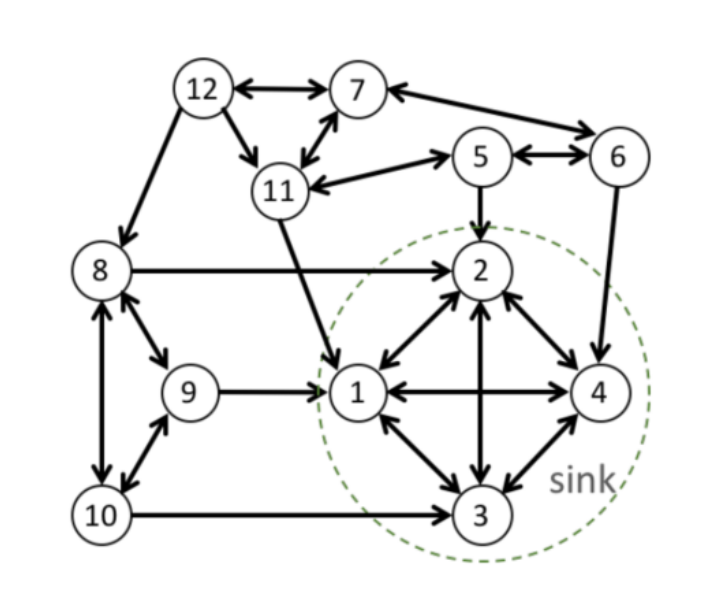
\includegraphics[scale=0.3]{Chapters/Figures/sink.png}
    \caption{A direct knowledge connectivity graph containing a sink}
    \label{fig:sink}
\end{figure}

However, the process of building the graph is quite complex in the sense that some properties must be guaranteed. In fact, the sink in the graph represents well connected nodes but that is not enough in which decentralized trust and fairness conditions must be ensured. This means that it is necessary to rotate the participants in the sink where each node has the same possibilities of entering the sink. Additionally, this model must not allow collusion of nodes and also it must be sybil resistant.

Based on the mentioned security properties, this model can then be applied to the consensus plane of permissionless blockchains. As a matter of fact, this model fits in the objectives of this dissertation in the sense that the main goal is to design a self adaptive consensus mechanism under the assumption of the \gls{CUP} model, therefore a possible solution will be discussed in chapter \ref{cha:elaboration-approach}.

% Basically, each node starts its execution with a few known participants of the system. Then, resulting of their execution, each node evolves and acquires more information about the system, and therefore, eventually reaching consensus.

%(inspired by short paper ...
%mas com o destaque que é preciso garantir condições de decentralized trust + fairness
%e não apenas nodes que estão num grafo coberto  ... que o modelo tem que ser
%tal que não pode haver colluison de gajos, os mesmos ou de sybil attacks.


%%%%%%%%%%%%%%%%%%%%%%%%%%%%%%%%%%%%%%%%%%%%%%%%%%%%%%%%%%%%%%%%%%%%%%%%%%%%%%%%%%%%
%%%%%%%%%%%%%%%%%%%%%%%%%%%%%%%%%%%%%%%%%%%%%%%%%%%%%%%%%%%%%%%%%%%%%%%%%%%%%%%%%%%%
%%%%%%%%%%%%%%%%%%%%%%%%%%%%%%%%%%%%%%%%%%%%%%%%%%%%%%%%%%%%%%%%%%%%%%%%%%%%%%%%%%%%

% \section{Scale-out scalability in different Blockchain Architectures}
% \label{sec:rel_work:scaleout}
% 
% \todo{side chain: parecido a multichain sem partilha de estado entre chains}
% 
% So far, we discussed different solutions and research methods to improve performance in \gls{DL}s in order to achieve higher transaction's throughput. However, this approaches are limited by not being to scale-out. Next we present 3 approaches that are able to achieve this kind of performance, namely Sharding, Multi-chains and Parallel chains. 
% Up to now, we discussed different solutions and research methods to improve performance in \gls{DL}s that includes modifying the chain's data structure or using multiple consensus mechanisms with the possibility of applying classical algorithms in order to achieve higher transaction's throughput. However, this performance improvements are limited and are not able to scale-out. Next we present 3 approaches that are able to achieve this kind of performance, namely Sharding, Multi-chains and Parallel chains. 


\section{Critical Analysis}
\label{sec:rel_work:critical_analysis}

Throughout this chapter we analysed different consensus mechanisms (section \ref{sec:rel_work_dl_scale_consensus}), some of them based on committees and how to apply them in permissionless blockchains. We have seen solutions that employ hybrid consensus planes in which \gls{PoW} serves as a mean to elect a committee of nodes to participate in the consensus of blocks, usually using \gls{PBFT}. We also discussed several scalability approaches that aim to improve \gls{DL}'s performance. In section \ref{sec:rel_work:dl_ds}, we presented an analysis of chained structures like Bitcoin \cite{bitcoin} and Bitcoin-NG \cite{bitcoin-ng} and the consistency problems of forks. We also, analysed different scalability solutions covering a wide spectrum from \gls{DAG} models, Sharding, Multichains and Parallel chains.

In relation to \gls{DAG} models, we concluded that solutions based on this approach can be divided in \gls{DAG} Block oriented or Blockless types. Although those solutions improve performance, some are vulnerable to liveness attacks \cite{block_dag, phantom_dag} or provide a weaker form of consistency \cite{spectre_dag} that prevents the support of smart contracts, which in our solution is a must. Regarding Sharding, we came across solutions that are able to scale-out by dividing the state across all nodes \cite{omniledger, rapid_chain}. Multichain solutions that allows to load-balance transaction processing to different systems and Parallel chains consisting of multiple blockchain instances which increases the rate of finalized blocks.

% chained structures like Bitcoin and Bitcoin-NG \cite{bitcoin, bitcoin-ng} and the consistency problems related to forks which also impacts on the performance of this type of systems. In order to mitigate the wasted resources of invalid blocks due to forks, the \gls{DAG} Block Model was presented as a way to incorporate the transactions of those blocks into the heaviest chain. However, solutions based on this model are vulnerable to liveness attacks \cite{block_dag, phantom_dag} or provide a weaker form of consistency \cite{spectre_dag} that prevents the support of smart contracts.

% Although the previous approaches increase the performance of \gls{DL}s they are not able to scale-out. In Section \ref{sec:rel_work:scaleout}, we presented $3$ mechanisms that are able to scale horizontally: 1) Sharding in which the system state is divided into multiple shards that can be executed independently and in parallel, but it is limited due to coordination of multiple shards which is slower than proposing a block in a single chain; 2) Multi chains that allows to exchange digital assets between different platforms while load-balancing transaction processing, but at the cost of building inter-chain secure protocols; and 3) Parallel chains that consists of multiple blockchain instances, although they are dependent on the smallest chain to finalize blocks.





In section \ref{sec:rel_work:adversary_model-consensus-consistency}, we discussed different consensus types and consistency guarantees which comprise the \gls{IC} protocol. When referring to \gls{PoW} or \gls{PoET} consensus mechanisms we concluded that their implementation is simpler but at the cost of reducing the throughput of the \gls{DL} in order to ensure an acceptable ratio between the rate of proposed blocks and their transmission, thus ensuring safety properties of the system. On the other hand, we analysed solutions that are based on committees like \gls{PoS} and \gls{PBFT} which are able to achieve a higher throughput of transactions by delegating the validation procedure to the committee, so the remaining nodes perform a more lightweight validation.

However, when applying committee based consensus to permissionless blockchains, it is necessary to perform a fair, trustable and sybil resistant \cite{sybil_attack} election based on a randomized process. Additionally, the committee must be refreshed in order to resist committee corruption attacks. In section \ref{sec:rel_work:sybil_committees}, we have seen the \gls{PPoS} variant based on committees employed by Algorand \cite{algorand_scaling_bft_cryptocurrencies} in which the election corresponds to a \textit{Cryptographic Sortition} process that leverages \gls{VRF} that when applied to the stake of the participants generates a committee. Additionally, the use of classical algorithms like \gls{PBFT} improve significantly the performance of the system. However, in the current state-of-the-art there are no solutions to permissionless blockchains that apply a hybrid and flexible Consensus Plane with the \gls{PBFT} mechanism, being a research challenge in which one of the possible approaches is based on the \gls{CUP} model \cite{cup_model}, presented in section \ref{sec:rel_work:cup}.

Next chapter, we present our elaboration approach that consists on building a \gls{DL} based on a Hybrid and Flexible Consensus that targets the \gls{CUP} model to support the \gls{PBFT} consensus mechanism. We believe that a solution that aggregates multiple consensus mechanisms can benefit from the tradeoffs of each one, thus achieving higher performance.
% when applied in different points of the execution of the system, thus achieving higher performance.
 